\section{Results}
Below the results from the experiments mentioned in \S\ref{sec:exp-setup} are outlined. Specifically, there are two main experiments that were run: the noise filtering experiment and the graph embedding dataset. As will be seen, the performance of both the Beta model and Normalizing Flow model exceeds that of GNNExplainer and provides additional information into the edge mask distribution. Note that in \cite{yuan_explainability_2021} and \cite{lin_generative_2021}, both GNNExplainer and PGExplainer demonstrate similar performance with their implementations coming from \cite{fey_fast_2019}. PGExplainer was unable to run on these examples with all predictred edge masks being very close to zero and demonstrating poor performance as a result. Hence, GNNExplainer is considered to be representative of the state of the art for the purposes of this work.

\subsection{Noise Filtering Experiment Results}
Note that for the following table, any prediction that was in the original graph structure is automatically given a correct. As mentioned before, since the goal of this experiment is not to determine the actual ground truth, but rather, to determine the ability of the explainer models to filter noise. For this experiment each of the methods was fed 25\% of the nodes that have noisy edges as a test and the results were collated. Not all nodes had noisy edges because of the probablistic noise sampling mechanism, but on average 50\% of the edges were noisy. This methodology means that the interpretation methods were exposed to slightly greater than 50\% noise as all nodes with no noise were filtered out.

As can be seen from the results in table \ref{tab:noise-filter-res}, GNNExplainer underperforms compared to both the Beta Model and the Normalizing Flow Model. The results indicate that all methods are doing a decent job at ensuring that noise is not picked up as important to the model. While there is room for improvement across the board, all methods demonstrate favorable performance with the bayesian learning methods leading the way in performance.
\begin{table}[htb] 
	\centering
	\begin{tabular}{|c||c|} \hline
	Model & Accuracy\\ \hline \hline
	GNNExplainer & 0.923\\ 
	Beta Explainer & \textbf{0.982}\\ 
	Normalizing Flow Explainer & 0.966\\ \hline
	\end{tabular}
	\caption{Accuracy results for all three models in the noise filtering experiment}
	\label{tab:noise-filter-res}
\end{table}

In particular, the Beta Model performs the best with the Normalizing Flow Model following it. While the Normalizing Flow Model is strictly more expressive than the Beta Model, it seems to exhibit higher variance in its training which leads to it picking up noise at times. This means that the Beta Model will perform better in experiments like this. Indeed, the restrictiveness of the Beta Model means that it would be more reluctant to pick any edge as positive. This probably explains its comparative advantage in this experiment and as will be shown later, the Beta Model is very good at picking out first-order pathways that are the most important to the GNN. While it may miss some information that is captured by the Normalizing Flow Model, this means that it is very good at filtering noise. 

The probablistic approach to both the Beta Model and Normalizing Flow Model means that they are better suited for filtering noise as compared to GNNExplainer which experiences little penalty for picking up a noisy edge as it tends to have little effect on the performance of the GNN. Instead, GNNExplainer cares much more about finding the postive edges and has little incentive for dropping noisy edges as demonstrated in the GNN performance from figure \ref{fig:tree-model-sparsity} where the noisy edges added little value but did not decrease the performance of the model. In the probabilistic models, though, these edges add little value and are discarded due to their minimal effect on the model which is discovered when the edge is both sampled and not sampled. 

\subsection{Graph Embedding Experiment Results}
With a known and confirmed groundtruth in this experiment, the interpretation methods were run through a few different metrics: accuracy, precision, recall, f1 score, and AUROC. In this case, the interpretation methods were compared directly against the groundtruth and the results were averaged across nodes to get the final results as seen in table \ref{tab:graph-embed-result}.
\begin{table}[htb]
	\centering
	\begin{tabular}{|c|c||ccccc|}\hline
	Model & Aggregation & Accuracy & Recall & Precision & F1 Score & AUROC \\ \hline\hline
	GNNExplainer & Avg Metrics & & & & & \\
	Beta Explainer & Avg Metrics & & & & & \\
	NF Explainer & Avg Metrics & 0.625 & 0.453 & 0.391 & 0.398 & 0.608 \\ \hline
	GNNExplainer & Avg Mask & & & & &\\
	Beta Explainer & Avg Mask & & & & &\\
	NF Explainer & Avg Mask & 0.667 & 0.333 & 0.400 & 0.364 & 0.672 \\ \hline
	\end{tabular} 
	\caption{A summary of results from the graph embedding experiment}
	\label{tab:graph-embed-result}
\end{table}

Based on these results, we can see that 

\subsubsection{Beta Model Edge Mask Distribution}
Additional, insights can be drawn about the GNN by looking at the distribution of edge mask values that the Beta Model came up with. In figure \ref{fig:tree-model-beta-marginal}, one can see the marginal distributions of edge mask values for each edge in the groundtruth. 
\begin{figure}[htb]
	\centering
	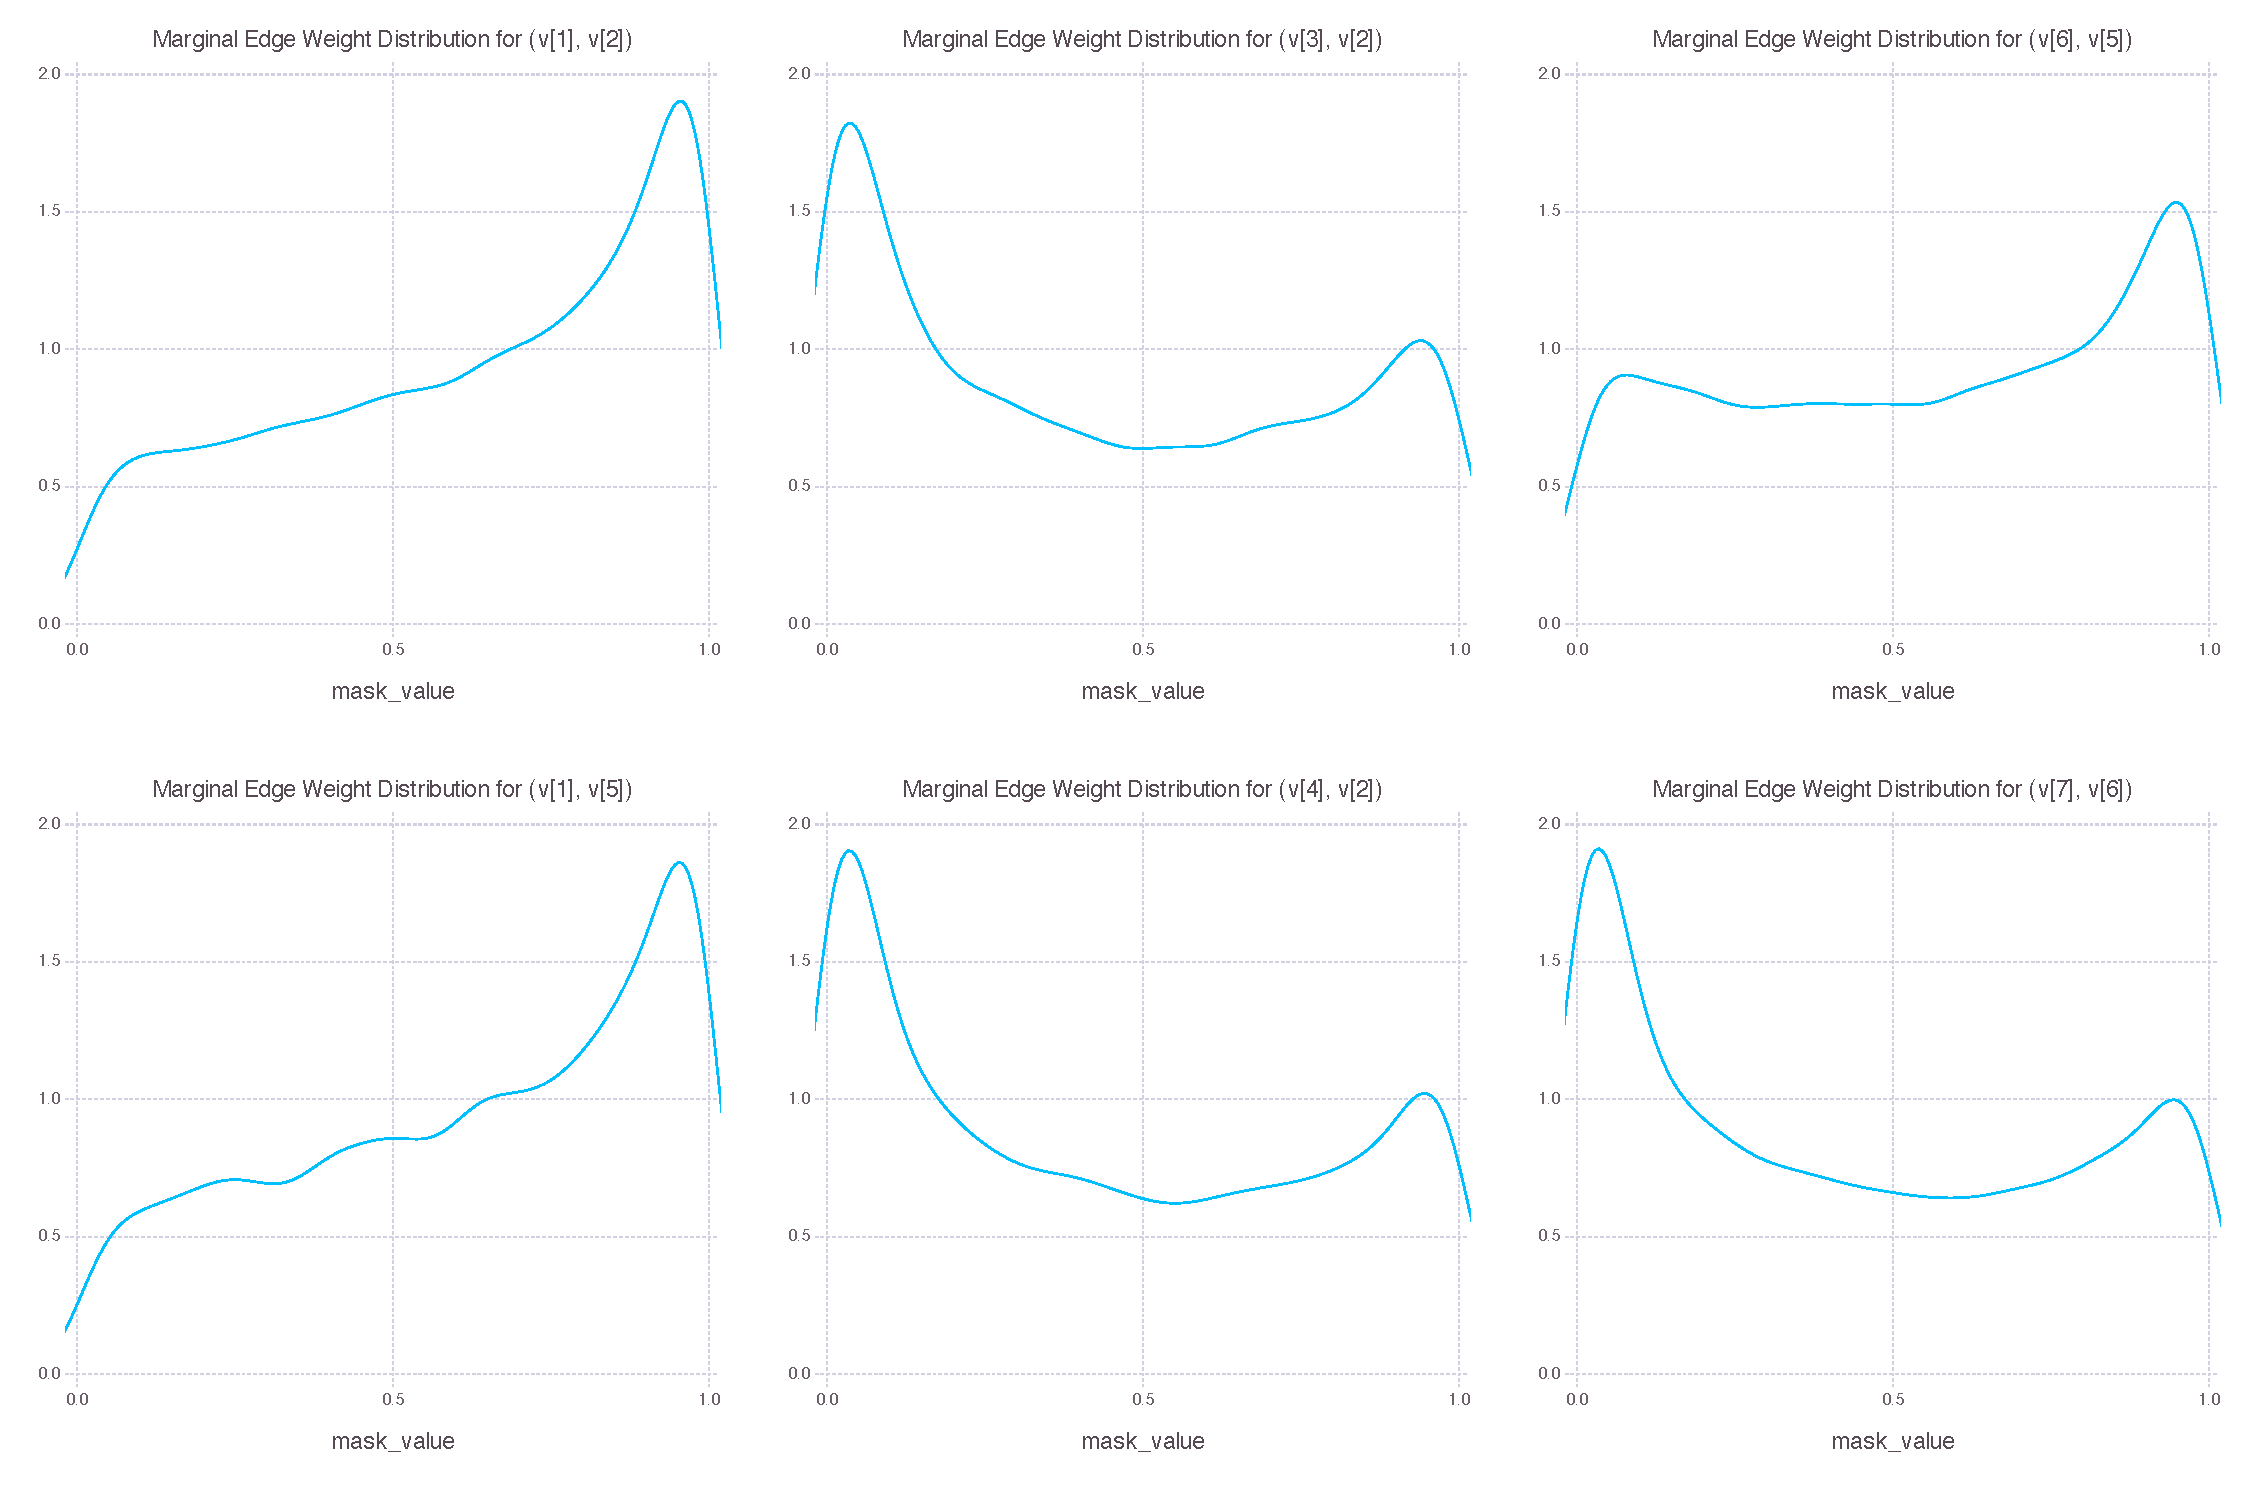
\includegraphics[width=0.8\textwidth]{images/tree-model-beta-marginal.pdf}
	\caption{Marginal edge weight distributions of all groundtruth edges in the beta model for a particular training point}
	\label{fig:tree-model-beta-marginal}
\end{figure}
From these marginal distributions, it is clear that messages coming out and into node 1 are highly important and that flows from node 6 to 5 are also highly important. The rest of the edges are not considered important. Note that this is for this particular example and not in general. This makes sense, though as a concentration of density in node 5 would force the model to focus on that region. Since the variational posterior is quite inflexible, the analysis from this model can be quite confident but shallow as it will only highlight the most important pathways.

Furthermore, insights can be drawn by looking at the joint distribution between pairs of edges. This can give insight into what edges are correlated, anti-correlated, and how many modes there are to the edge mask distribution. This is important as it gives researchers insights into the different mechanisms that drive performance in the GNN. If the GNN is being used in a physical sciences or biology context, for example, this can help elucidate the various mechanisms that map to physical phenomenom. As seen in figure \ref{fig:tree-model-beta-joint}, the Beta Model helps provide a great first order approximation to these types of pathways.
\begin{figure}[htb]
	\centering
	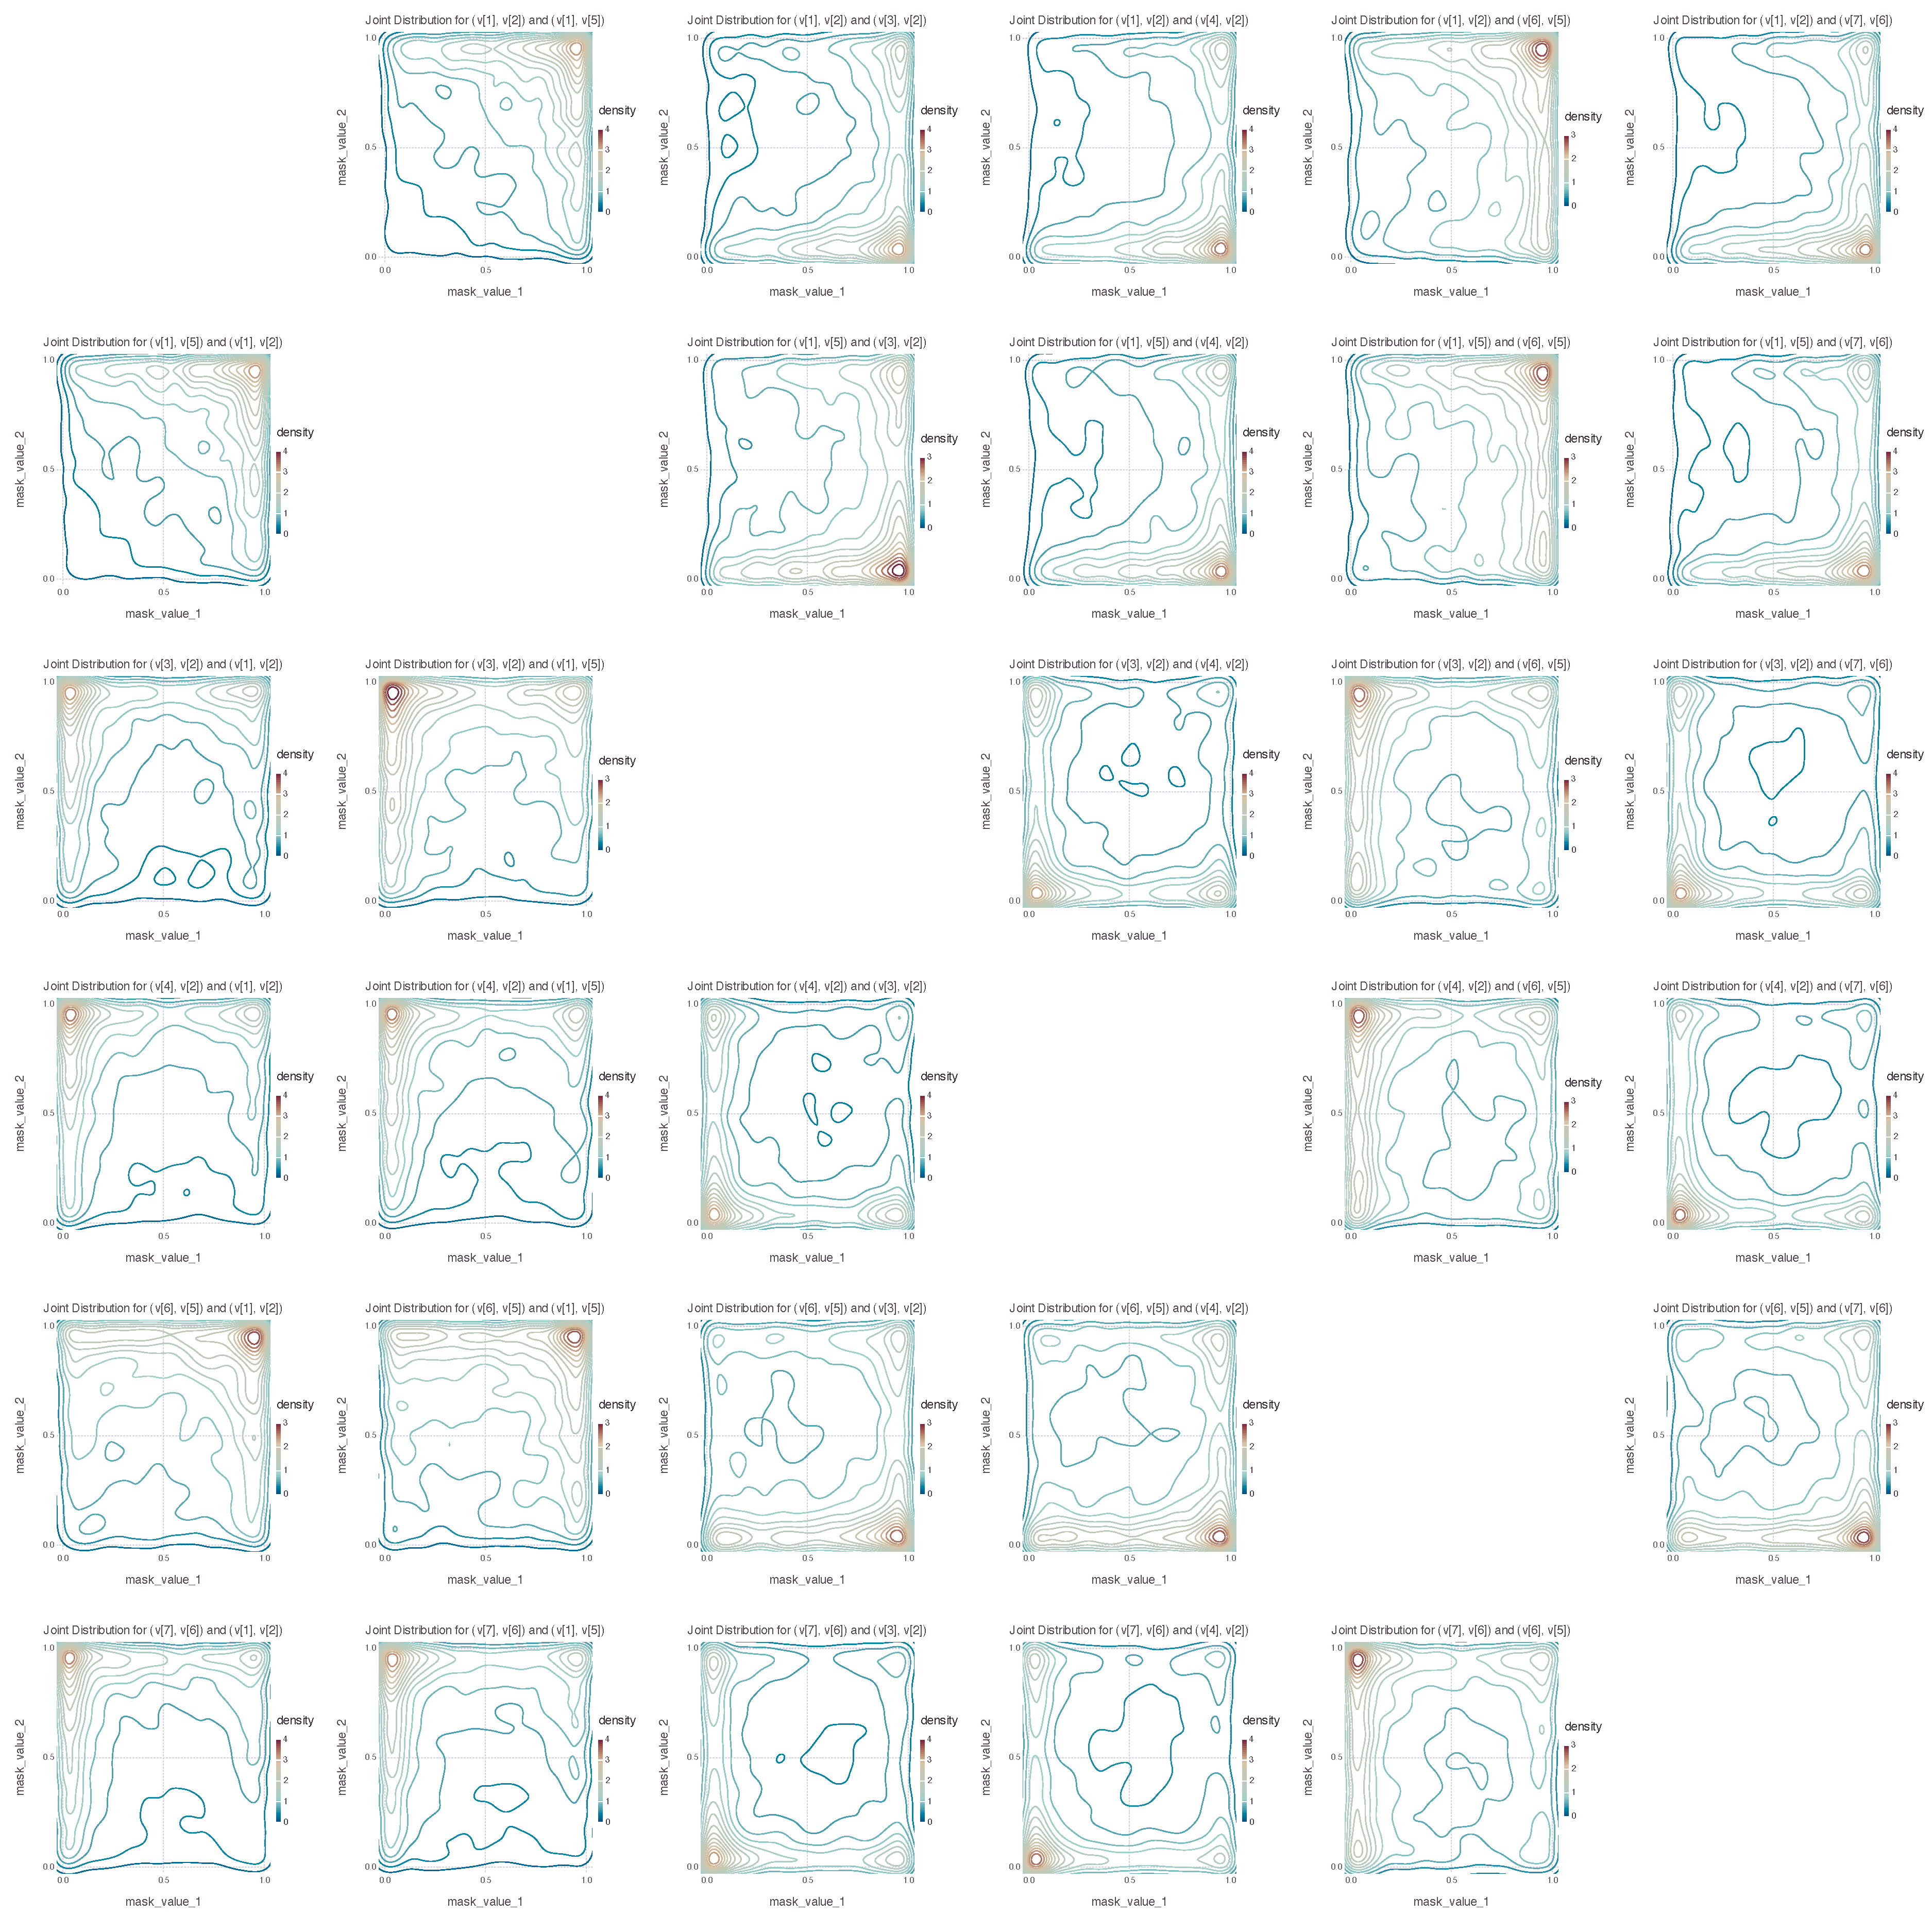
\includegraphics[width=0.8\textwidth]{images/tree-model-beta-joint.pdf}
	\caption{Joint edge weight distributions between pairs of groundtruth edges in the beta model for a particular training point}
	\label{fig:tree-model-beta-joint}
\end{figure}

Specifically, by looking at the joint distributions of edges, one can tell when a certain pair of edges is postively coorelated, negatively correlated or lacks any correlation at all. In figure \ref{fig:tree-model-beta-joint}, looking at edges $3 \rightarrow 2$ and $1 \rightarrow 5$ demonstrates that for this example, the model is certain that edge $1 \rightarrow 5$ is important while the edge $3 \rightarrow 2$ is not. Perhaps this is due to an accumulation of density in node 5 while there was not as much sampled at node 2. Indeed, this can be coroborrated by looking at $6 \rightarrow 5$ and $1 \rightarrow 5$ where both are very positively correlated and indicates that information is pooling at this node for this particular example. Finally, it is clear that bidirectional flows from node 1 and its neighbors are highly important as well. Overall, this gives a great unimodal intuition about the way in which information flows through the model.

\subsubsection{Normalizing Flow Model Edge Mask Distribution}
A similar analysis can be done for the Normalizing Flow Model. Note that this model is much more flexible than the Beta model which gives it a higher variance but allows it to capture multiple different pathways and local minima that the GNN may experience. This can already be seen in the marginal distributions as seen in figure \ref{fig:tree-model-dnfg-marginal}.
\begin{figure}[htb]
	\centering
	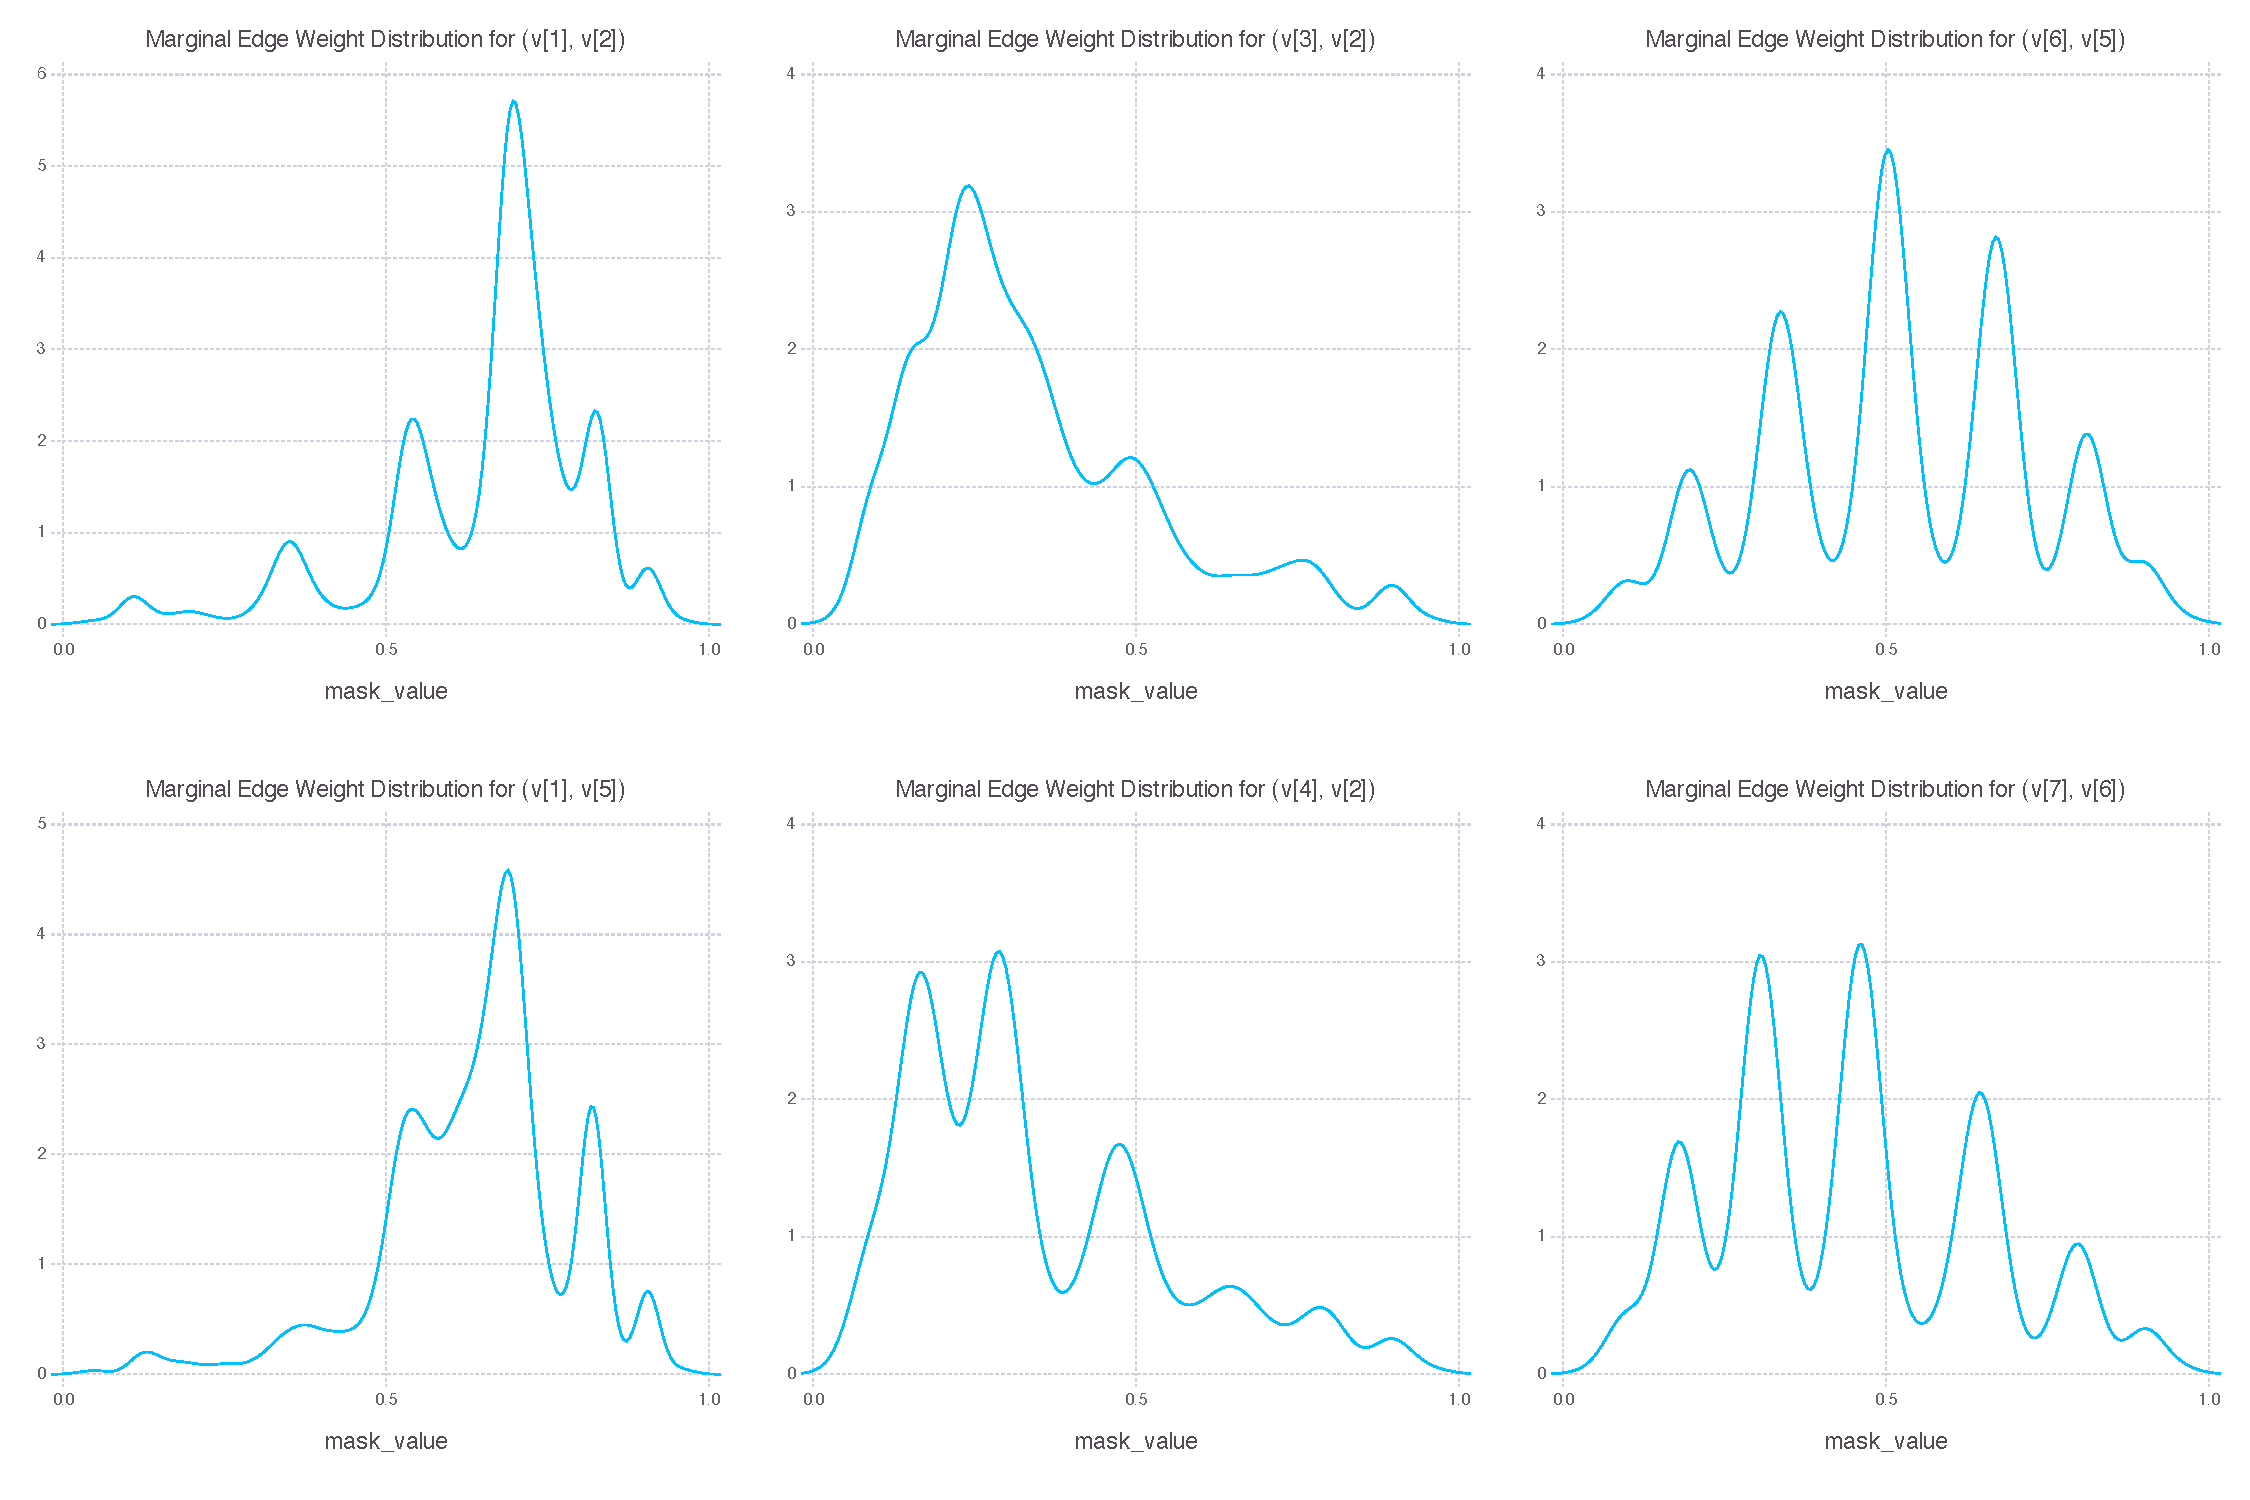
\includegraphics[width=0.8\textwidth]{images/tree-model-dnfg-marginal.pdf}
	\caption{Marginal edge weight distributions for all groundtruth edges in the normalizing flow model for the same training point as \ref{fig:tree-model-beta-marginal}}
	\label{fig:tree-model-dnfg-marginal}
\end{figure}

Indeed, 

As with the Beta Model, the joint distribution between pairs of edges helps illustrate an even richer tale as seen in figure \ref{fig:tree-model-dnfg-joint}.
\begin{figure}[htb]
	\centering
	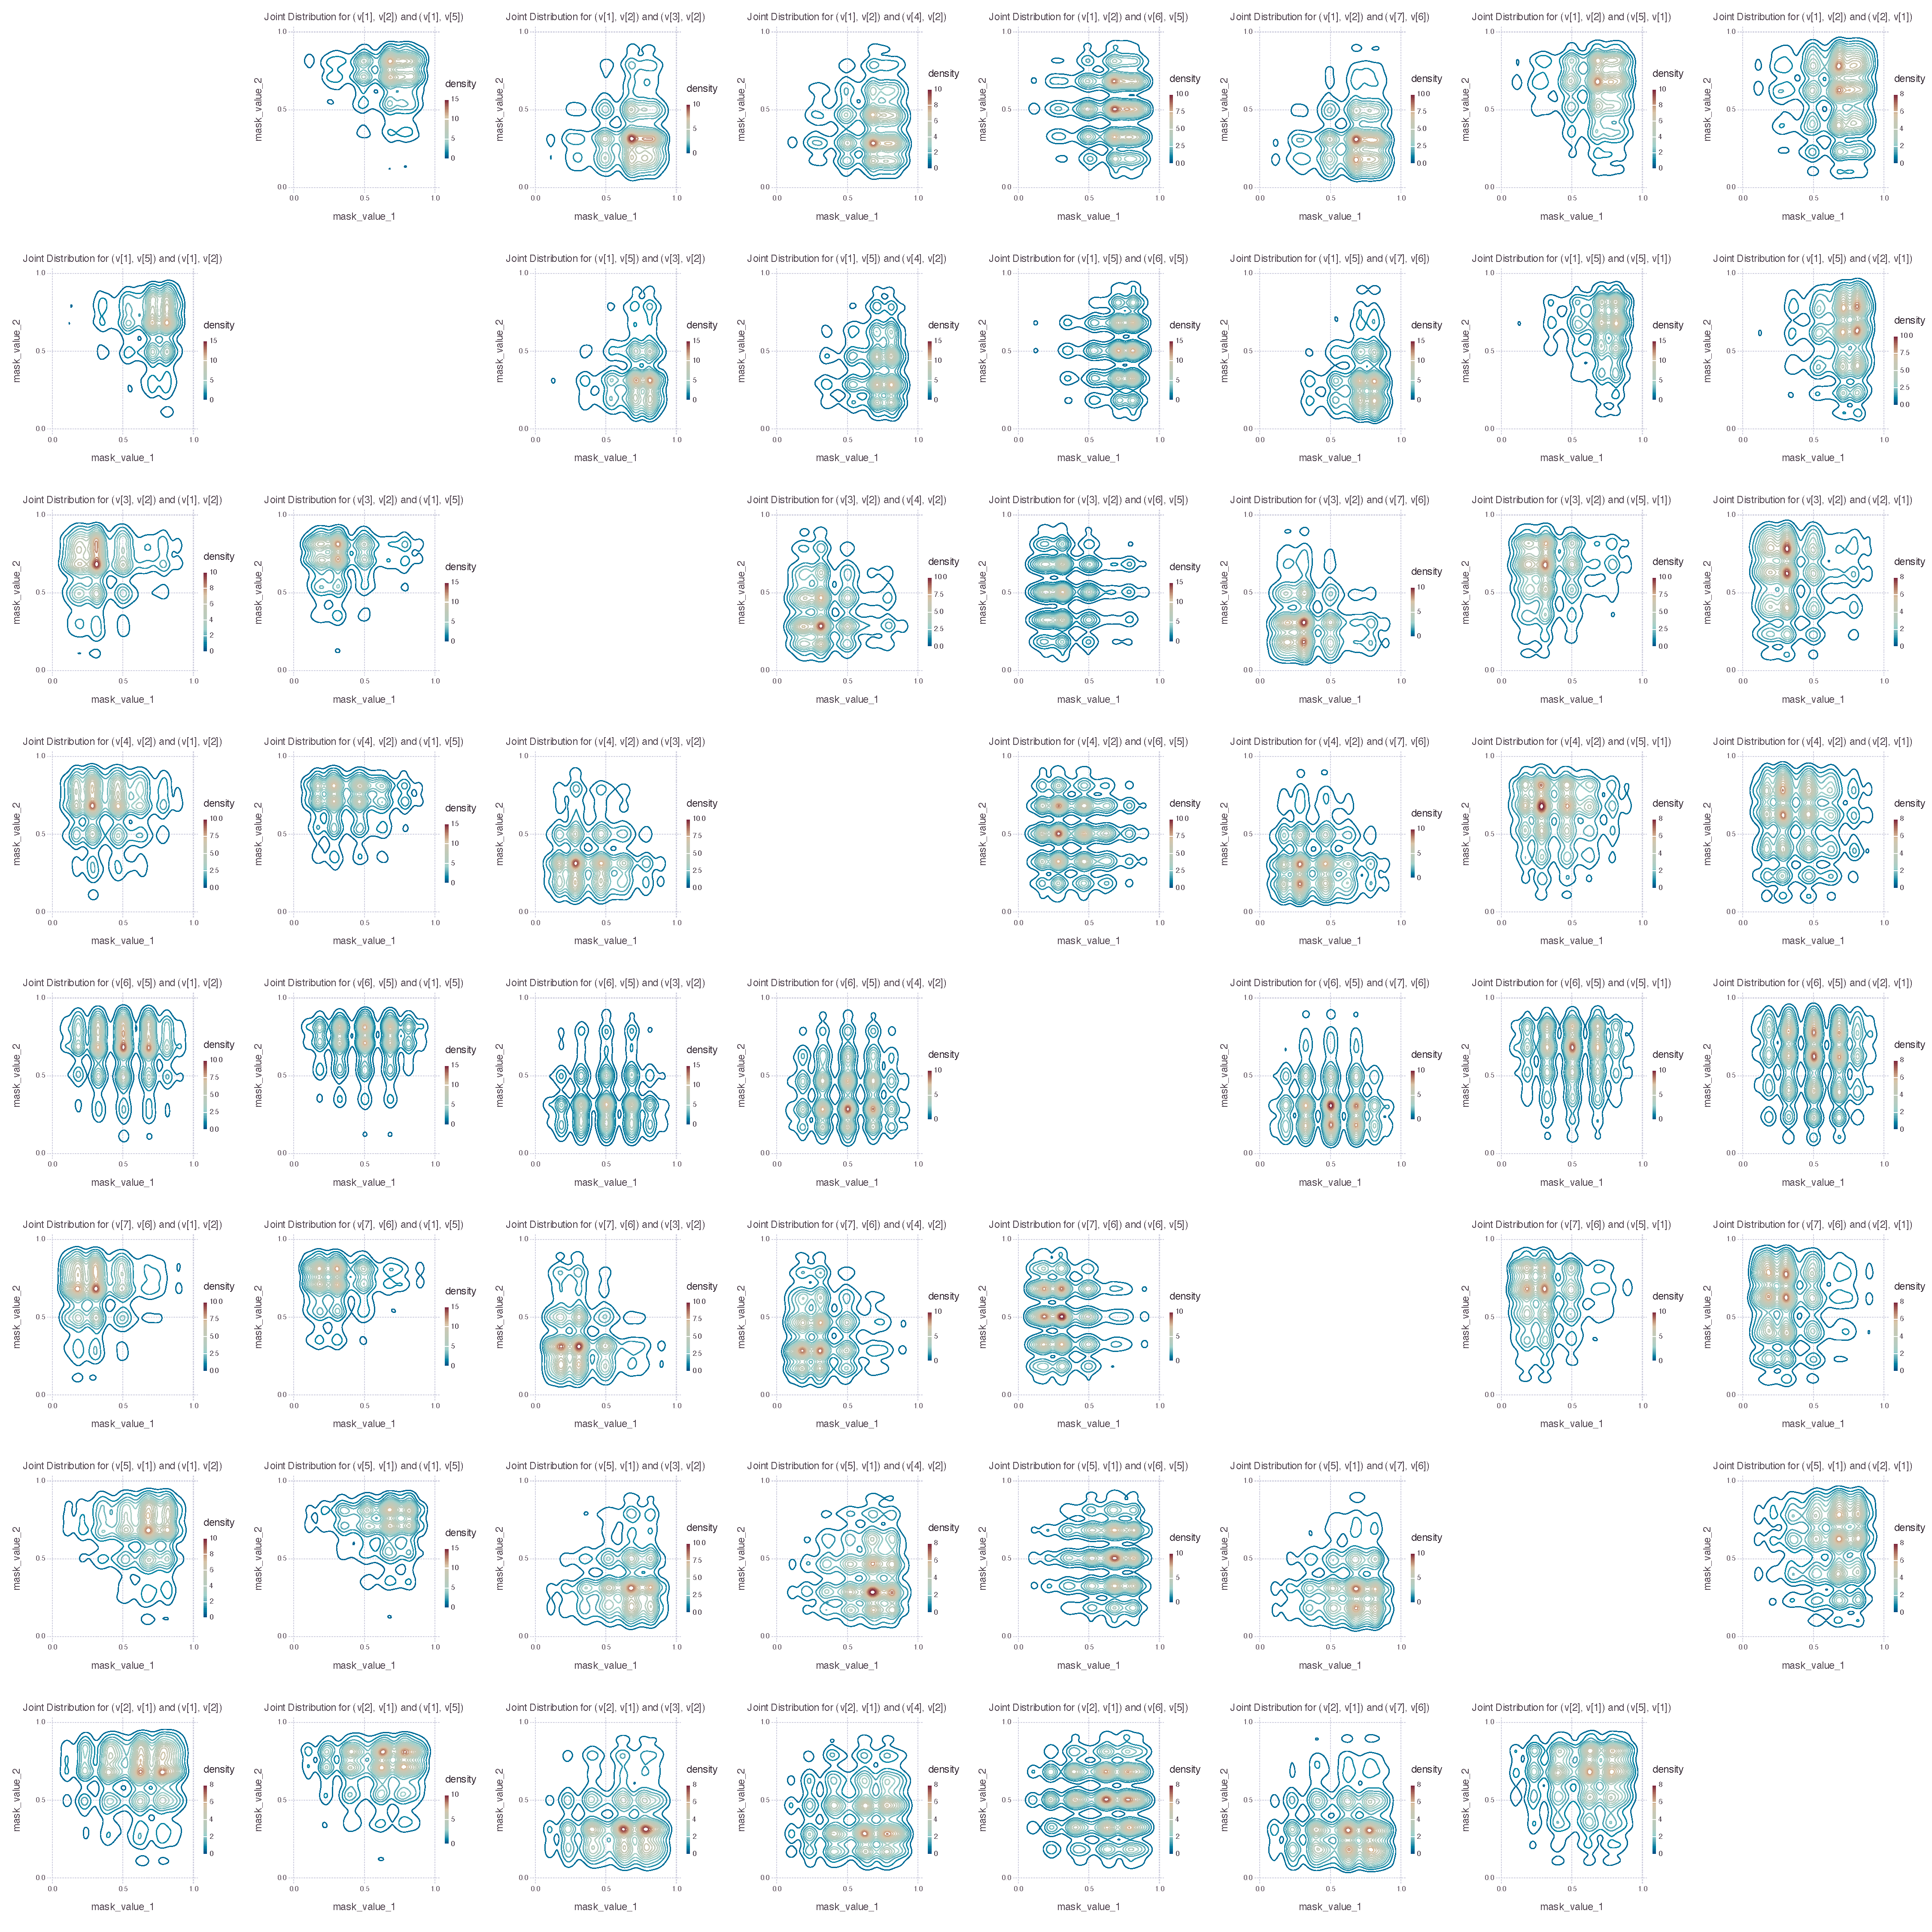
\includegraphics[width=0.8\textwidth]{images/tree-model-dnfg-joint.pdf}
	\caption{Joint edge weight distributions between pairs of groundtruth edges in the normalizing flow model for the same training point as \ref{fig:tree-model-beta-marginal}}
	\label{fig:tree-model-dnfg-joint}
\end{figure}

For example,

\newpage
